% ---------------------------------------------------------------------
% EG author guidelines plus sample file for EG publication using LaTeX2e input
% D.Fellner, v1.17, Sep 23, 2010


\title[NetVis Network Traffic Visualization]%
      {NetVis: A network traffic visualization tool}

% for anonymous conference submission please enter your SUBMISSION ID
% instead of the author's name (and leave the affiliation blank) !!
\author[Nicholls et. al.]
       {James Nicholls, Dominik Peters,
       	Albert Slawinski, Thomas Spoor, Sergiu Vicol, Jassim Happa
%        S. Spencer$^2$\thanks{Chairman Siggraph Publications Board}
        \\
% For Computer Graphics Forum: Please use the abbreviation of your first name.
         Department of Computer Science, University of Oxford
%        $^2$ Another Department to illustrate the use in papers from authors
%             with different affiliations
       }

% ------------------------------------------------------------------------

% if the Editors-in-Chief have given you the data, you may uncomment
% the following five lines and insert it here
%
% \volume{27}   % the volume in which the issue will be published;
% \issue{1}     % the issue number of the publication
% \pStartPage{1}      % set starting page


%-------------------------------------------------------------------------
\begin{document}

% \teaser{
%  
\includegraphics[width=\linewidth]{eg_new}
%  \centering
%   \caption{New EG Logo}
% \label{fig:teaser}
% }

\maketitle

\begin{abstract}
   Computer network traffic visualizations attempts to deliver improved understanding of traffic on a network to an observer. 
Many existing tools opt for graph or plot-based visualizations to detect patterns or outliers in the data, but still largely
provide a segmented view of any data feed. In this paper, we present a novel network traffic visualization framework that 
makes use of a variety of complementary visualizations to obtain better situational awareness. 
Our proposed solution is to look at different..

\begin{classification} % according to http://www.acm.org/class/1998/
\CCScat{Computer Graphics}{I.3.3}{Picture/Image Generation}{Line and curve generation}
\end{classification}

\end{abstract}

\section{Introduction}
Analysing and monitoring network traffic is an important part of network security. Since the amounts of data involved in this task are extraordinarily large, it can be hard to make effective use of them. Visualizations offer a solution: they give a compact representation of data to a human analyst who can use them to detect patterns in the network \cite{ware2012information}. An effective visualization of network traffic makes it easy to identify outliers while making clear the general patterns of network usage, and it will facilitate detection of intrusions and malicious activity.

In this paper, we present a set of visualization techniques that work in tandem to improve awareness of activities in ongoing network traffic passing through an analysts systems. They have been implemented in a robust application to provide an analysis framework for 
network activity in an interactive manner, enabling a deeper and more straightforward understanding of the data. Two of the visualizations are based on existing literature (parallel coordinate plots \cite{inselberg1985plane} and spinning cube of potential doom \cite{cube04}), whereas the four remaining visualizations are novel to this paper. These are referred to as: Attribute Distribution, Traffic Volume, Heat Map and Activity Groups.  

Time series data in the form of packet captures are processed in real-time and simultaneously rendered in multiple connected visualizations. The user can switch between the available representations of the data and change both the visualization's layout and the amount and type of the data displayed. The software is designed to make it easy to spot irregular activity and investigate it from multiple perspectives.

The framework aims to provide an environment in which situational awareness can more effectively be obtained. It is therefore flexible to the demands of the specific situation. New visualizations will in a natural way complement the existing ones: The underlying data processing engine provides a standard data basis which is shared by all displays.

The tools emphasize exceptions, show comparisons, and answer a wide variety of questions in a concise fashion. We want the user to generate good hypotheses in response to the visualized information. To achieve this, aids are given to the user to avoid cluttering displays with irrelevant data. In particular, we have implemented a filtering system which can be adjusted in response to changing situations.

Though the application's main purpose is to monitor current activity in the network, the same architecture can be used to forensically analyse recorded data. The system simulates the data records as if they represent a live network. This exploits the important dimension of time and makes it easier to understand recorded activity.


\section{Related Work}
JH

\section{NetVis Architecture}
\textbf{Add information on CSV, Data, non-existence of analysis of packet content, and add info on data flow through the application.}

Normalisers:
A normaliser is a class responsible with taking a packet and returning a ``normalised'' value of a certain attribute of that packet and the other way around. The Source IP normaliser provides a method that takes a packet and returns a value between 0 and 1 corresponding to its Source IP (0.0.0.0 returns 0, 255.255.255.255 returns 1). It is also capable of taking a value from 0 to 1 and returning a human readable IP address. 
Each normalising class is able to create a temporary filter in the application that will filter its corresponding attribute on a certain range. 
Since the normalising class is in control of its filter it can create a zooming effect based on the value of the filter. 
(If there is a filter on the Source Port normaliser from 0.5 to 1 then port 30000 will be normalised to ~0 instead of ~0.5.)
// You can extend this + make it pretty

Filtering:
\textbf{High-level: What do filters do?}
The application supports two types of filters - filters that the user explicitly defines, and filters applied on-the-fly from within the visualisations.
Both types are applied to all visualisations and information displayed, and can be adjusted at any time without losing prior data.
The user has access to a variety of different filter controls.  First, there is a menu for filtering by transit protocol. By default, all protocols are selected and therefore included. Protolcols are sorted into menus by protocol family, appearing in multiple places where appropriate. Second, there is a control to select the range of ports the application uses, which defaults to the maximum port range.  The source and destination ports can be set separately, enabling a user to view all data entering/exiting a port as desired.  Next, there are IP and MAC address filters.  These work on a blacklist/whitelist system, allowing a user to only view packets to or from a particular set of addresses, or ignore packets going to or from a different set.  This enables a user to, for instance, ignore traffic from sources they know are irrelevant or focus only on an address that is causing concern.
The second type of filter will be dealt with in more detail in sections 4.2 and 4.3.

Modularity: \textbf{[Make this better.]}
The application was designed to be very extensible.  Adding a new visualisation is simply a matter of adding it to the application's list of those available, which will cause it to be included and kept up-to-date as packets come in and are filtered.  The same is true for filters and normalisers.  \textbf{[wrong place:] }Adding a filter would result in its controls automatically being included in the right panel and all packets would then be filtered according to the criteria it specifies.  Adding a normaliser would cause it to be integrated with the Spinning Cube, Dataflow and Attribute Distribution visualisations.  Ths modularity extends even so far as data input.  If a class were written to accept packets from a different source, it would be trivial to switch the application to use this class.

\section{NetVis Visualizations}
The user interface of the application focusses around the displayed
visualization, which takes up the majority of the window, and can be maximised
to fill the available space. Other panels occupy the right and bottom sections
of the window, and are as follows.

Choice of visualization is presented to the user by a list in the top of the
right panel, followed underneath by options specific to that visualisation, and
then by general filters to refine the processed data. Lastly, time controls are
included on the right panel to allow the user to fine-tune the speed at which
data is processed and displayed. The right panel is ultimately aimed at
providing the user with options to adapt the shown data.

The function of the bottom panel is to show fine and aggregate details of the
processed data. To fit the large amount of data available into such a limited
space, a tabbed pane is used on the left to categorise distinct types of data.
The right section of this panel contains a `Context Pane', the purpose of
which is to show even further detail of selected data on demand. The left
`Analysis' panel and the right `Context' panel are split in two by a split
pane, so the user can modify the proportion of each they wish to see.

Less-frequently used program functions, as well as window tools, are included
in the form of a main menu bar. Common window tasks are available via the menu
bar, as well as an exclusive-mode full screen option and the facility to select
a new data source.

Messages to the user come in the form of warning dialogues for user or program
errors, notifications in the bottom `Analysis' panel for program notifications,
and text messages in the bottom `Context' panel for help messages and
suggestions. A diagram of the application layout is included below.

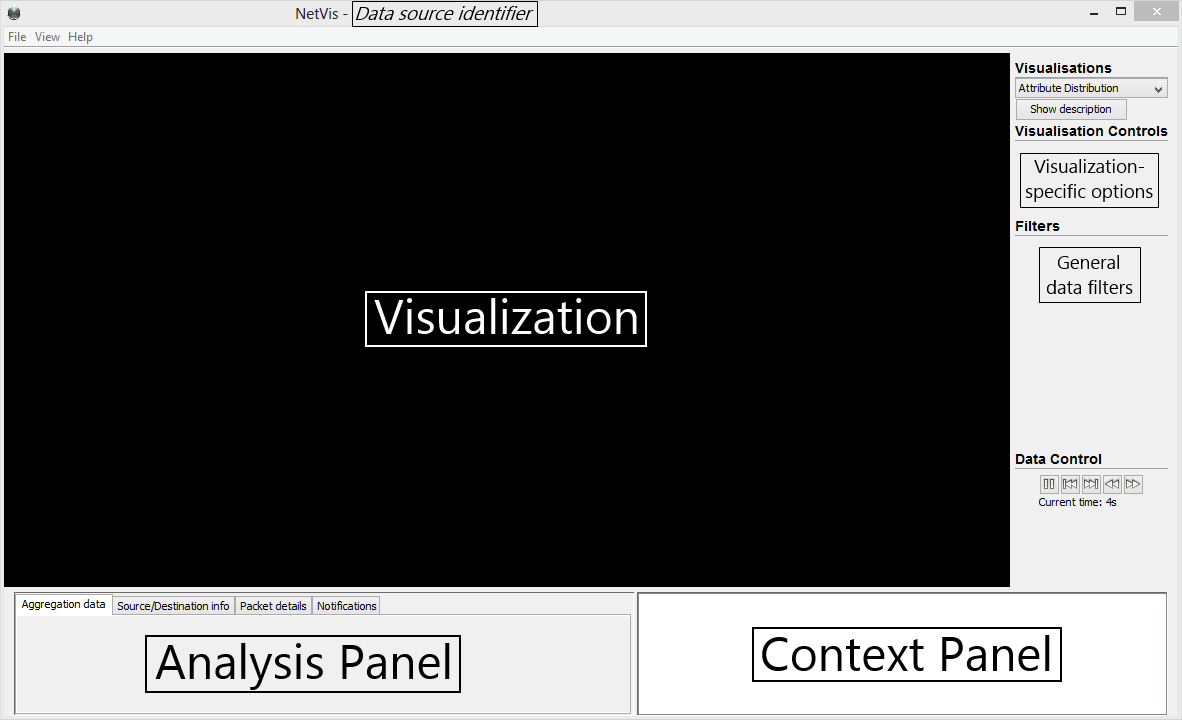
\includegraphics[width=\linewidth]{materials/layout-diagram.png}


\subsection{Attribute Distribution}
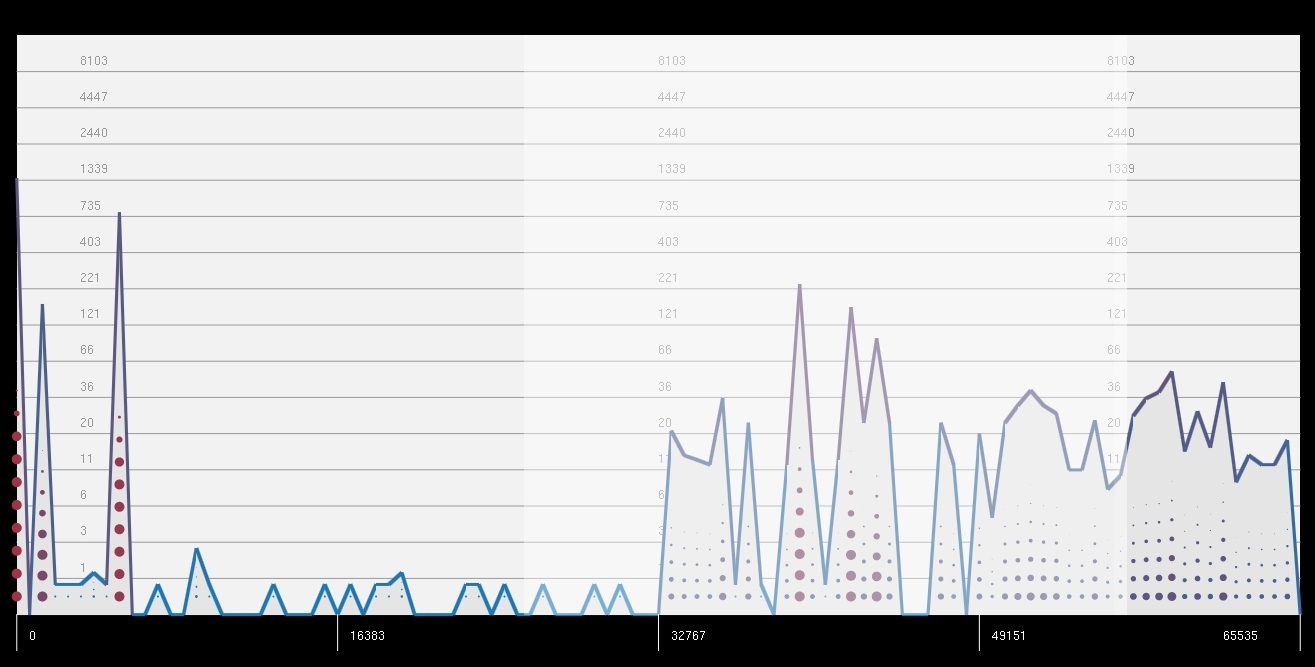
\includegraphics[width=\linewidth]{materials/distribution.jpg}

The most common need in the analysis of network traffic is to get information on the distribution of certain features of the packets. For the graph constructed here, the user selects such a feature (e.g., ports or destination IPs). A logarithmic line graph is then drawn, and (as with all visualizations in the application) updated in real time. A logarithm is applied to assist in detecting spikes.

A second layer of the visualization is presented to the user simultaneously: Circles under the line graph indicate the actual distribution (without a logarithm applied) through their area. Furthermore, all lines and circles are colour-coded to give extra signals of the volume of traffic. Red elements are under heavier load.

All these features have a single purpose: make the analyst understand what is going on, and to make obvious any anomalies.

This visualisation makes active use of the normalisers described above. It also allows the user to click-and-drag along interesting data which then automatically applies a filter to the data so that all visualizations focus on this user-selected area of interest.


\subsection{Data Flow}
The Data Flow visualization applies the idea of parallel coordinates proposed by \cite{inselberg1985plane} to network traffic. Following the principles layed out in \cite{fliggnetwork} the visualization shows the `flow' of each packet, representing each as a line through the parallel coordinates. This provides an informative view of the whole traffic in the network. It visualises the distribution of various packet attributes while also giving an intuitive insight into relationships and correlations between distinct aspects of the packets.

Lines representing packets are coloured based on their value in some coordinate. They fade out based on how old the packet is, thereby placing focus on newer developments in the network. 

A common criticism of parallel coordinate plots is that they make it hard to interpret data that is uniformly distributed between coordinates or that is very concentrated around few values \cite{marty2009applied}. Our implementation addresses these concerns using animation. Lines representing new packets are randomly pertubed and move subtely. This makes it easier to spot whether a colourful line represents one or more packets. The animation allows the user to distinguish between single packets and concentrated groups of packets with the same characteristics.

For example, if multiple requests to a server came from a single MAC address through the same ports and using the same protocol, in a non-animated visualization they would all be represented by the same line. A user would erroneuosly interpret this as a single request. Adding randomness makes the pack of requests more visible without significantly impacting the accuracy of the data representation.

Hovering over one coordinate displays a scale for the attribute it represents. Clicking transfers you to the distribution visualisation showing the distribution of that particular attribute.


\subsection{Spinning Cube}
The Spinning Cube is an implementation of an existing visualization tool known as the spinning cube of potential doom\footnote{See \url{www.kismetwireless.net/doomcube/}}.
It�s displays packets as dots inside a spinning cube. Their 3D position is based on 3 packet attributes. (eg. x-axis $\Rightarrow$ Source Port / y-axis $\Rightarrow$ Destination Port / z-axis $\Rightarrow$ Source IP). The 3 coordinates are customisable.

\textbf{[make nicer]}


\subsection{Traffic Volume}
The Traffic Volume visualization is inspired by the `FlowScan' graph
(\url{www.caida.org/tools/utilities/flowscan/}). It is realised as a stacked
bar chart which displays the volume of data arriving in each time interval.
Each column is segmented into segments with heights proportional to the total
number of packets transmitted for each protocol.
In addition, the column segments are colour-coded and can be cross-referenced
with a protocol key underneath the visualization itself.

To help distinguish between different protocols, colours are selected from a
colour palette which provides colours from a qualitative colour scheme.
The objective of this visualisation is to allow users to see at a glance if a
particular protocol is being exploited in the network. The increase in both
column height and colour proportion should draw attention to any protocol which
becomes overburdened.

A control panel is provided in the right panel for the purpose of adjusting the
number of time intervals displayed at once on the x-axis. The y-axis scales
automatically to fit the relevant data.


\subsection{Heat Map}
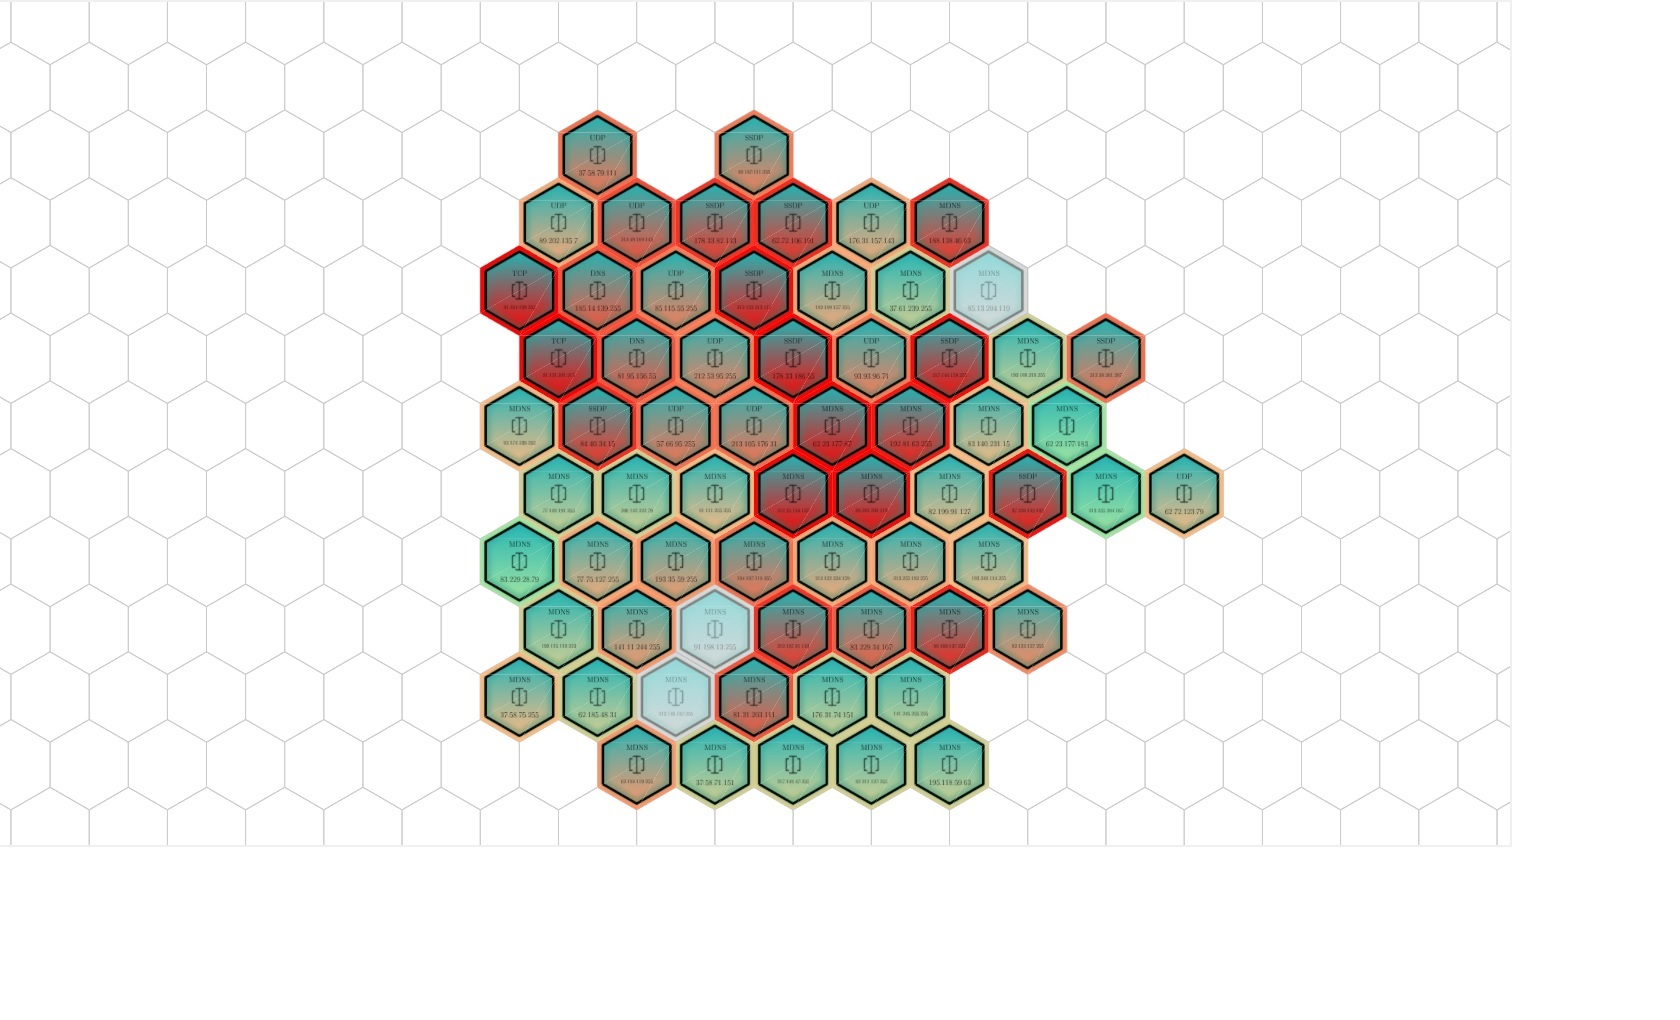
\includegraphics[width=\linewidth]{materials/heat-map.jpg}
The Heat Map visualization uses a hexagonal map to display a compacty cluster of nodes.
Each machine found to be communicating in the analysed network will be represented as a node.
The activity of a specific machine in the network is represented by the colour of the 
corresponding hexagon. As more and more traffic arises, nodes representing the machines that
send and reveive data ``heat up'' and, as the time passes, ``cool down''.
The hexagonal grid is being filled in a compact manner - new nodes are place outside of 
the already displayed nodes. The relative position of the map elements in this visualization
does not play a role on default. There is a way to sort the nodes so that they form a radial 
gradient - the more ``heated up'' will be sorted to the middle.

This visualization helps a user find machines that are most active in the network.
It gives a quick overview of the number of the clients and how many of them are currently active.
Additionaly every node presents some information, such as the machine's most commonly used protocol.
This lets users do some basic data selection choices easily. For example: if some other visualization
is being obscured by too much data from one specific machine, or too much data of some protocol,
the user can look at the heatmap and find out what filters to apply to make the overview of the situation
more clear.


\subsection{Activity Groups}
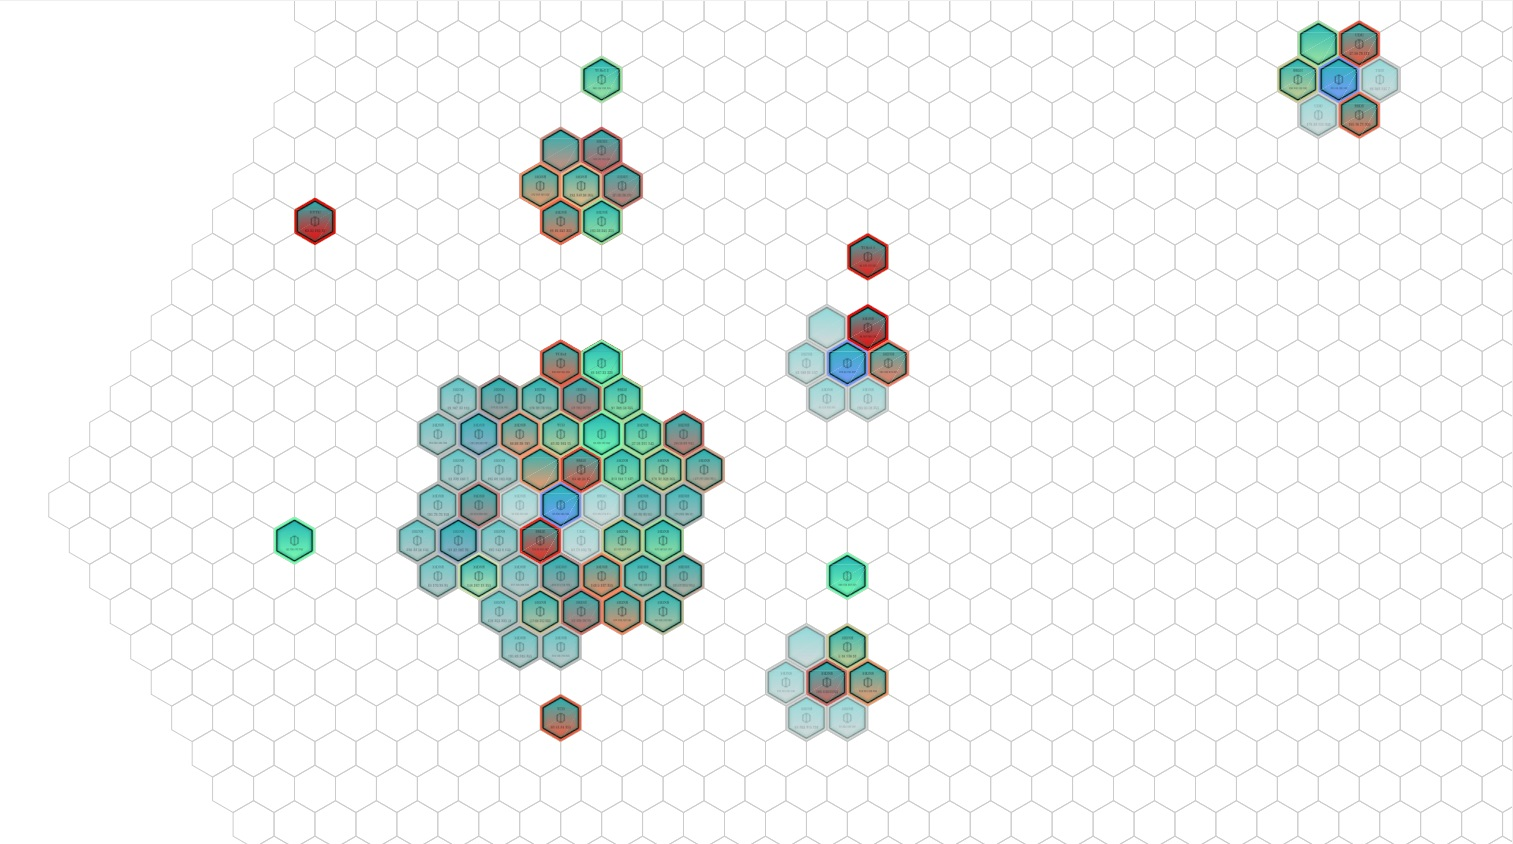
\includegraphics[width=\linewidth]{materials/groups.jpg}
Expanding on the hexagonal grid, this visualization employs two important visual factors:
size and proximity.

As the traffic in the network rises, the visualization groups together all the machines
sending packets to one specific device. As more and more machines communicate with a specific
address, more and more nodes appear around the hexagon representing that destination.

The colour of the communicating nodes represents how much data they send. More heavily used destinations 
will thus have more orange and red nodes around them, and destinations used by a lot of machines will have a greater number of nodes around them.

Node placement is automatic. The procedure ensures that there is enough space around a centre and that no two nodes overlap.

This visualization helps detect the machines that perform a server role in the network.
It also allows a user to quickly guess what type of service the device is providing. Each node specifies the
most commonly used protocol, thus revealing the possible role of the server node.

\section{Discussion}
The main determinants of traffic in a network are the network's topology, the flow of the traffic, and the type of the traffic. The graphical visualizations presented here ensure that the available data can be interpreted from all three of these perspectives. Moreover, the underlying idea of our design is that better insight into the activity in the network can be gained by combining these perspectives.

Each visualization was chosen to fill a specific purpose.  The Heat Map visualization fills the need to gain a very quick impression of overall network load and size.  The Activity Groups visualization provides the same information on a server-by-sever basis, providing more data at the expense of simplicity.  The Data Flow visualization provides the ability to see what the traffic of the network currently `looks' like, and the Spinning Cube and Attribute Distribution visualisations allow the user to detect pattern in the attributes of the packets.

Note that the visualizations combined here differ in their approach to handling the inherent multi-dimensionality of traffic data. An effective visualization framework needs to make clear how traffic changes as time progresses, and needs to show interesting developments in diverse attributes such as port use, source and destination machines, protocol use or traffic volume. Showing all this information simultaneously runs at the risk of obstructing the simplicity needed for ready understanding of a human observer. Our visualizations both use multi-dimensional systems (such as parallel coordinates) to give an overview, and use visualization with fewer dimensions but more detail. This encourages an understanding of network activity that is both broad and detailed.

To arrive at a complete understanding of the network, a single visualization will typically not be sufficient. An analyst will need to see different approaches to interpret the data, and will need to customize the visualizations and the data displayed in them. This is where the design principles of interactivity and interconnectedness of NetVis provide powerful assistance, and ensure that the visualizations in combination achieve both effectiveness and expressiveness \cite{mackinlay1987automatic}. 

\subsection{User Workflow}
From the perspective of an analyst examining a network, a typical workflow
would begin with considering all activity from a broad overview, using any
number of visualizations. Once a network attack has been identified, it should
be easy for the analyst to ``zoom in'' to the data of interest, by applying
successive filters to the source, and changing the representation to suit the
particular attack. Finally, when the exceptional behaviour has been singled
out, the analyst may explore details of the intrusion on demand.

This workflow illustrates the visual design framework suggested by Ben
Shneiderman, University of Maryland, in 1996;

\begin{center}
    \textit{Overview first, zoom and filter, then details-on-demand.}
\end{center}

To assist with the process of singling out suspicious activity, certain
visualizations allow filtering by mouse interaction. Where appropriate, the
analyst may click or drag their mouse cursor over sections of the active
visualization to create a new filter, or switch to a different representation
of the selected data. Navigation between complementing visualizations in this
fashion is highly intuitive and allows the analyst to tweak the active filters
quickly and effectively.

The following is a graphical representation of the typical workflow expected of
an analyst studying a network using NetVis.

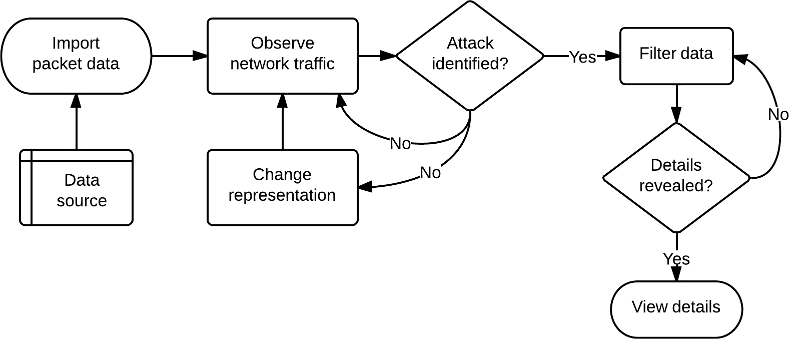
\includegraphics[width=\linewidth]{materials/workflow-diagram.png}


\subsection{Advantages}
Existing network visualization solutions are typically single-purpose programs which present given data in one specific way (see for instance the catalogue in \cite{marty2009applied}). The analyst is expected to choose in advance which kind of visualization will provide the most insight, and is then limited to what the specific application is able to show. Existing applications also require different input file formats which makes it complicated to use them simultaneously. % (for a discussion of these problems see ). 

The program presented here takes a single data input stream and simultaneously visualizes it in different presentations. Since these visualizations are built upon a common base, they are able to complement and inform each other. This improves the user's ability to investigate anomalies.

Network visualizations have to process and display a large amount of data. Often, this can cause a visualization to be cluttered and lose its effectiveness. An obvious solution is to provide filters which allow the analyst to focus on phenomena of interest. The filters we provide apply application-wide and can be defined in an intuitive manner from within the visualizations themselves in a ``click-and-zoom'' fashion. This is a significant improvement over existing workflows.

The framework developed here can be used both for real-time monitoring, but also for historical analysis, which makes it applicable for a wide variety of use cases. Furthermore, the application can be used as a learning tool: by observing archived data captures, new users can familiarise themselves with the general patterns of network usage, and can also see how suspicious patterns show up in a visualization.

\subsection{Limitations}
Doesn't use all data

\subsection{Future Work}
More advanced data processing
Machine Learning
Save current configuration and have access to sensible filter packages


\section{Conclusion}
We have presented a network visualization tool to analyse and monitor network traffic. Instead of presenting single perspectives (visualizations) of the data very well (but with a limited scope), our framework delivers a variety of visualizations that complement each other and work in tandem to help an analyst obtain improved awareness of ongoing network activity through user interaction. We overviewed its suite of visualizations and demonstrated its usefulness with example scenarios. In the future we intend to add more visualizations and further improve the tool's usability.


%-------------------------------------------------------------------------

\bibliographystyle{eg-alpha}

\bibliography{netvisbib}

\end{document}
